\section{Training und Hyperparameter}

%___________________________________________________________________
\begin{frame}{Einstellungen für das Training}

\textbf{Trainingsdaten:}
\begin{itemize}
    \item 49.000 Trainingsbilder, Größe $32 \times 32 \times 3$
    \item Batchgröße: 256
    \item DataLoader-Worker: 12 (hohe Parallelisierung)
\end{itemize}

\textbf{Training:}
\begin{itemize}
    \item Trainierbare Parameter: 604.810
    \item Iterationen pro Epoche: $\lceil 49{,}000 / 256 \rceil = 192$
    \item Epochen pro Trial: 10
\end{itemize}

\textbf{Hyperparameter:}
\begin{itemize}
    \item \alert{Bayesian Search} mit 20 Trials
    \item Optimierte Parameter: ch1, ch2, ch3, Lernrate, Weight Decay
\end{itemize}
\end{frame}

%___________________________________________________________________
\begin{frame}{Genauigkeit während des Trainings}
\begin{figure}
    \centering
    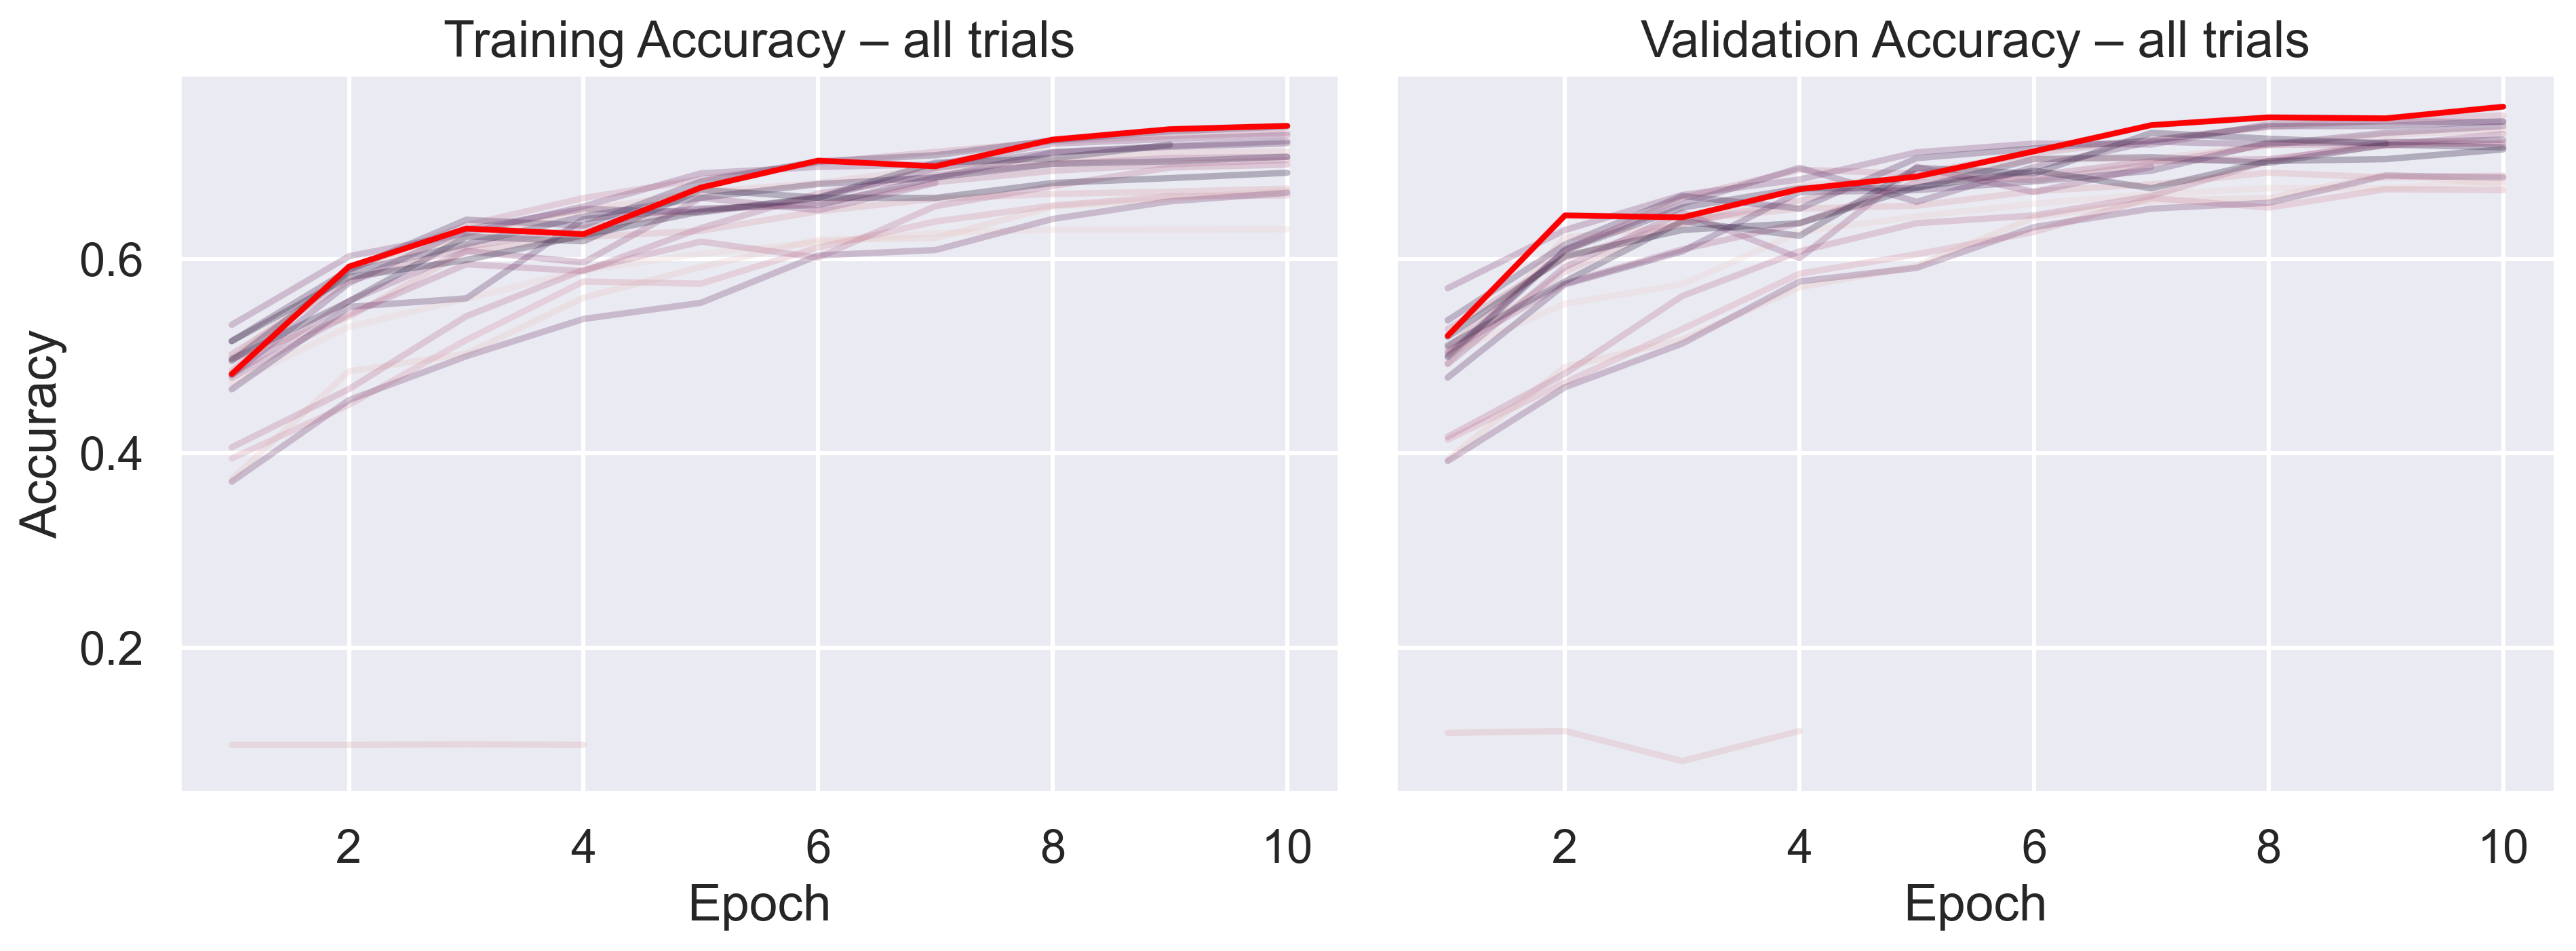
\includegraphics[width=\imagewidth, height=\imageheight, keepaspectratio]{all_trials_accuracy.png}
\end{figure}
\end{frame}

%___________________________________________________________________
\begin{frame}[fragile]{Early Stopping}
\textbf{Motivation:} 
\begin{itemize}
    \item Verhindert Overfitting
    \item Stoppt Training, wenn Validierungsgenauigkeit über mehrere Epochen nicht steigt
\end{itemize}

\textbf{Prinzip:}
\begin{itemize}
    \item Wähle Grenzwert: \texttt{patience}
    \item Nach  jeder Epoche: Behalte den besten Validierungswert
    \item Zähle Epochen ohne Verbesserung: \texttt{epochs\_no\_improvement}
    \item Stoppe, wenn \texttt{epochs\_no\_improvement $\ge$ patience}
\end{itemize}
\end{frame}

%___________________________________________________________________
\begin{frame}{Hardware-Auslastung}
\begin{columns}[T,onlytextwidth]

    \column{0.45\textwidth}
    \textbf{Hardware:}
    \begin{itemize}
        \item GPU: RTX 4060 Ti, 16 GB VRAM
        \item CPU: Ryzen 5 7600X, 12 Kerne
        \item RAM: 32 GB DDR5
    \end{itemize}

    \column{0.55\textwidth}
    \begin{figure}
        \centering
        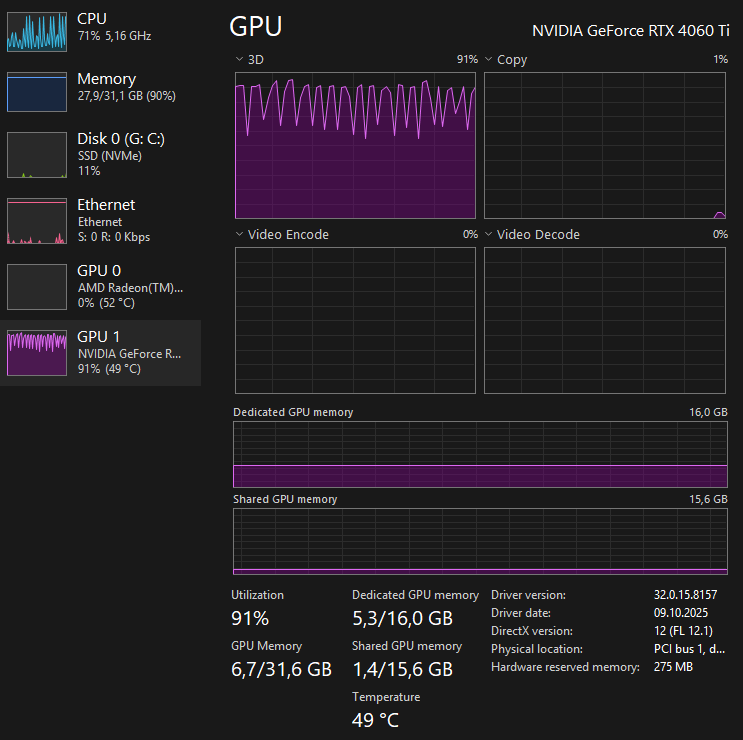
\includegraphics[width=\linewidth, height=0.8\textheight, keepaspectratio]{machine.png}
    \end{figure}

\end{columns}
\end{frame}


%___________________________________________________________________
\begin{frame}{Laufzeiten pro Trial}
Gesamtdauer: ca. 15 Minuten

\begin{figure}
    \centering
    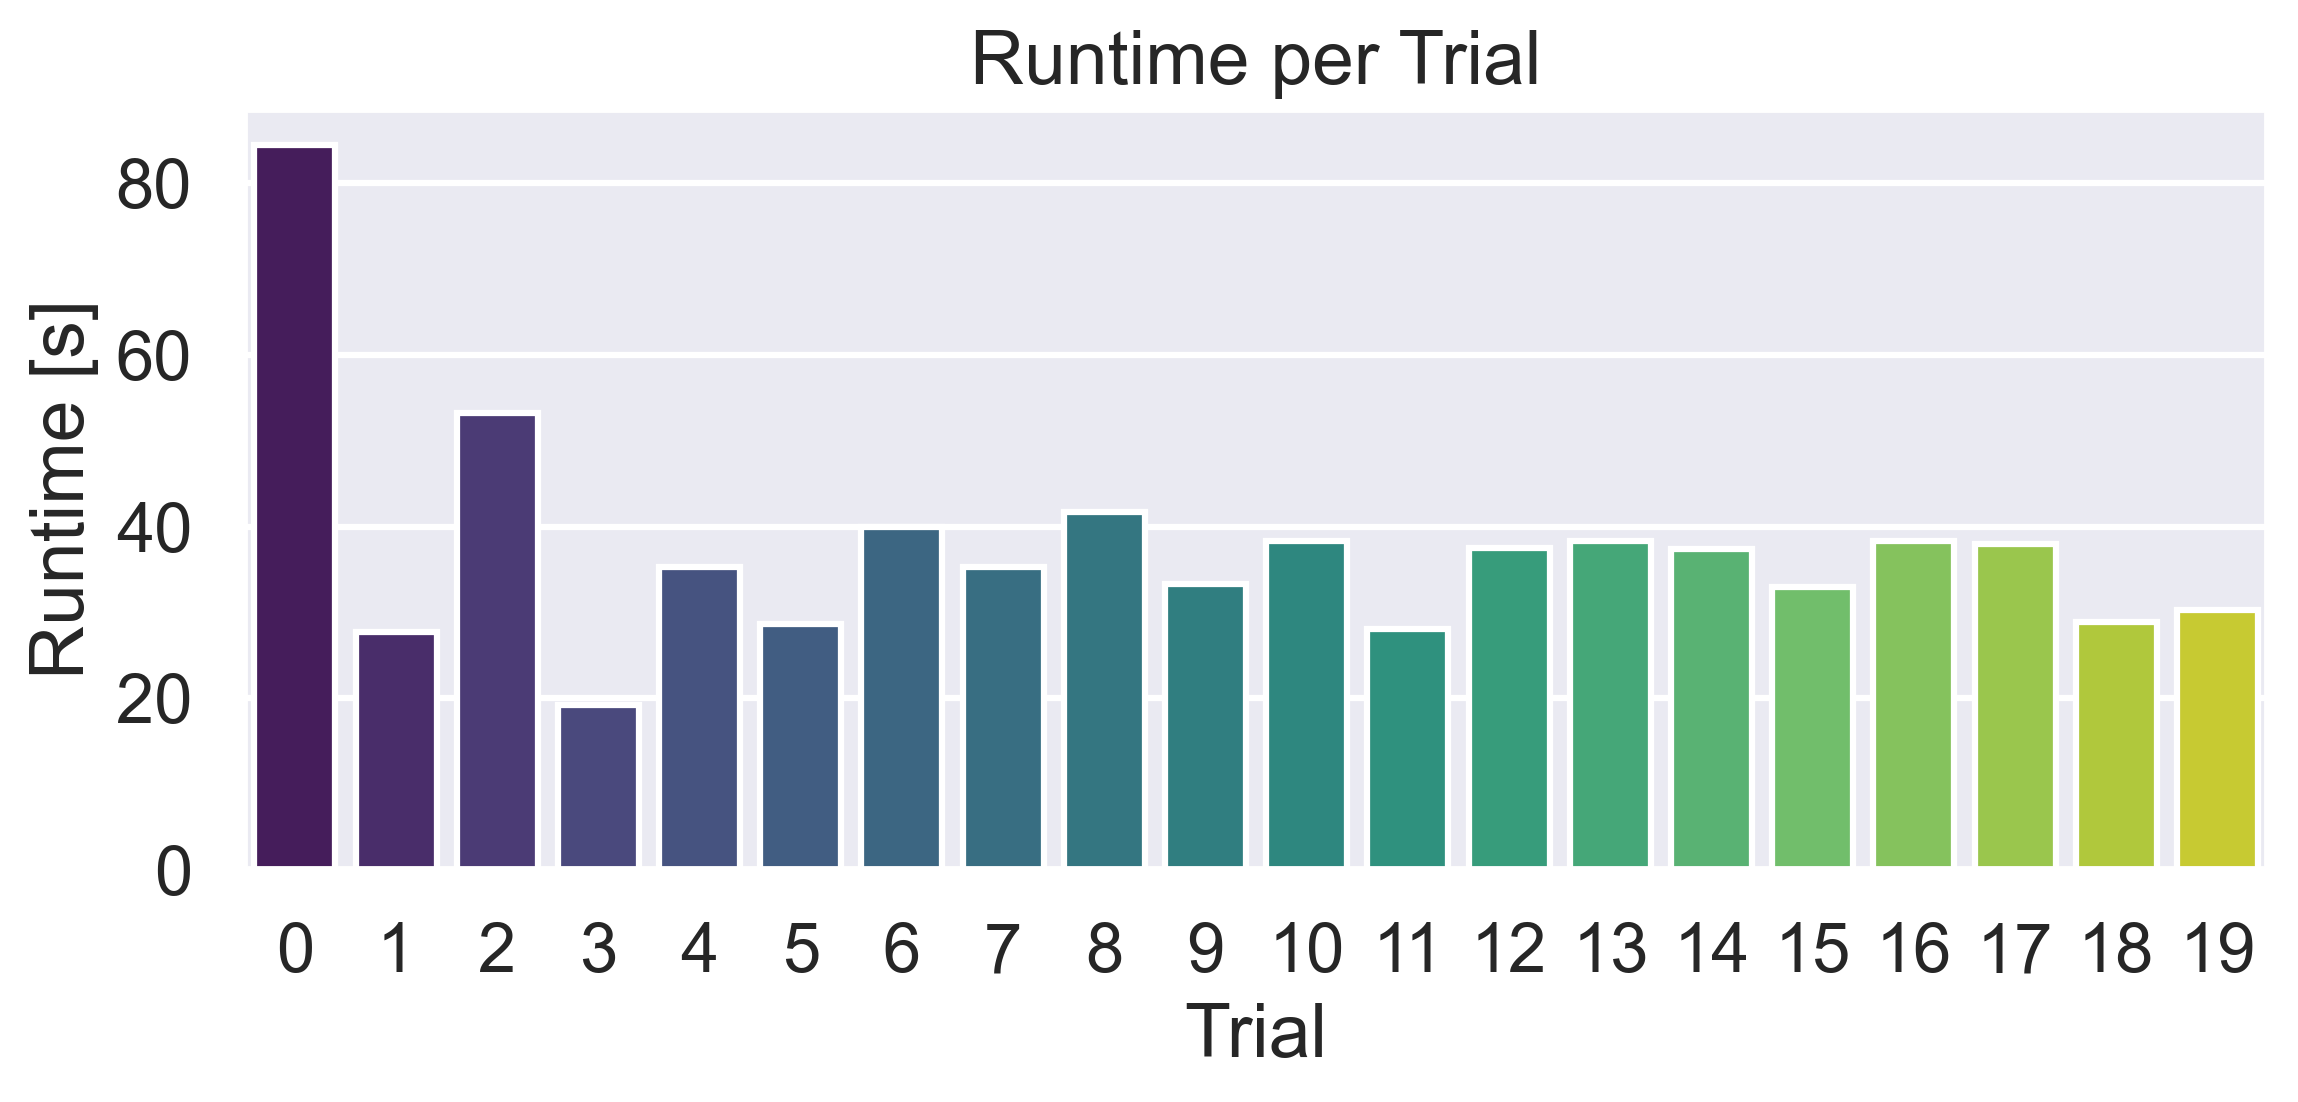
\includegraphics[width=\imagewidth, height=0.8\imageheight, keepaspectratio]{runtime_per_trial.png}
\end{figure}
\end{frame}
